%------------------------------------------------------
\begin{figure}[!t]
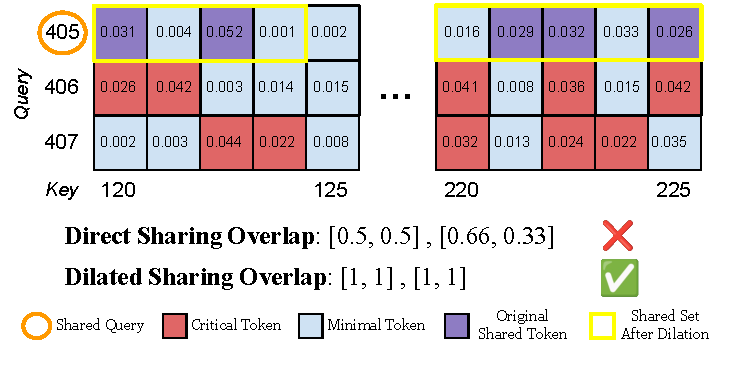
\includegraphics[width=0.48\textwidth]{assets/index-frag.pdf}
\centering
\vspace{-0.5em}
    \caption{\textbf{Critical-index set (CIS) dilation.} For three adjacent queries (405–407), we examine two key-index clusters $[120,125]$ and $[220,225]$. Critical tokens from query 405 are shared to queries 406 and 407. Overlap is measured as $\frac{\text{Number of True Positive}}{\text{Number of Critical Tokens}}$. Tokens in \textcolor[HTML]{A64DFF}{violet} are also critical for query 405.}
    \label{fig:index-frag}
    \vspace{-1em}
\end{figure}
%--------

\vspace{-0.05in}
\section{Proposed Method and Implementation}
\vspace{-0.05in}
\label{sec:method}

In this section we present CPE. First, \textbf{CIS} (from Observation~1) enables efficient head-level KV sharing across adjacent queries. Next, \textbf{PSAW} and \textbf{ETF} (from Observation~2) prune redundant attention by shrinking visible attention window and freezing early token updates, respectively, with theoretical error guarantees. We also describe CUDA kernels for parallel index manipulation and sparse attention.



\subsection{Clustered Indices Sharing (CIS)}
\label{sec:cis}

CIS performs head-level KV sharing with dilated shared set among semantically similar, and temporally adjacent queries. By \textbf{Observation}~1 and \textbf{Theorem}~\ref{the:mean-shift}, the critical clusters for such queries undergo only small mean shifts relative to a reference query. Therefore, exhaustive per-query head-level retrieval is unnecessary. We first partition the sequence into fixed-length blocks and restrict sharing to within a block to enforce temporal adjacency, where semantically similar but non-adjacent (cross-block) queries are not shared. 


\paragraph{Selection Criteria}
Within each block, the first query serves as an initial reference and computes its critical indices across layers and heads. Following~\cite{zhang2023h2o,wuhshare} and the locality bias in \textbf{Observation~2}, selection budgets are allocated to three token groups: initial (sink) tokens, local tokens, and salient middle tokens. Let $C_{\text{sink}}$ and $C_{\text{local}}$ denote the numbers of sink and local tokens, respectively. At decoding step $t$, we obtain the middle set with a budget $k$ by applying the top-$k$ oracle over positions $[C_{\text{sink}}, t\!-\!C_{\text{local}}]$, excluding the sink and local regions. This yields $S_t^*=\{p_{t,i}\}_{i=1}^{k}$, where $p_{t,i}$ is sorted and selected in descending order of attention weight. The per-head critical index set is $\mathcal{C}_t=\{1,\ldots,C_{\text{sink}}\} \cup S_t^* \cup \{t-C_{\text{local}}+1,\ldots,t\}$, with a total size $C=C_{\text{sink}}+k+C_{\text{local}}$.




\paragraph{Similarity Criteria}
For a later query, if there exists an earlier query $j$ whose cosine similarity exceeds a threshold $\tau$, KV sharing is performed. We measure similarity as
\begin{equation}
\begin{aligned}
\label{eq:cos_sim}
\mathsf{sim}(i,j)=\frac{\bq_{i}^{\!\top} \; \bq_{j}}{\|\bq_{i}\|\,\|\bq_{j}\|}.
\end{aligned}
\end{equation}
If multiple candidates satisfy $\mathsf{sim}(i,j)>\tau$, we choose the most recent such $j$ to preserve adjacency. Varying $\tau$ trades throughput for accuracy.

\paragraph{Neighboring Dilation}
Naive sharing ignores centroid drift (Eq.~\eqref{eq:centroid_shift}) and yields fragmented critical sets (Figs.~\ref{fig:attn-cluster}, \ref{fig:index-frag}), missing true positives for shared queries. We therefore dilate the $m$ highest-weight indices in $S_t^*$ (with $m\!\le\!k$) by their $\pm r$ neighbors:
\begin{equation}
\label{eq:neighboring}
\begin{aligned}
\hat S_t 
\;=\; 
S_t^* 
\;\cup\;
\bigcup_{i=1}^{m}\big\{p_{t,i}+j \;|\;-r\le j\le r\,\big\}.
\end{aligned}
\end{equation}
As shown in Fig.~\ref{fig:index-frag}, dilation substantially increases true-positive overlap and achieves complete coverage compared to direct sharing. Moreover, restricting dilation to the top-$m$ indices mitigates attention pollution from adding excessive low-weight tokens, as detailed in Sec.~\ref{sec:cis-dilation}.

\paragraph{Analysis}
\label{sec:cis_analysis}
Theoretically, CIS also turns Property~\ref{prop:among-query} into a pre–hoc guarantee as proved in Theorem~\ref{thm:cis-main} (detailed in \textbf{Appendix A, A3}). 

\begin{theorem}[CIS Retained–Mass and MI Guarantee]
\label{thm:cis-main}
For a reference query $q$ and its shared set $\hat S_t$ dilated with $\pm r$ neighbors 
around the top-$m$ winners ($m<k$), as in~\eqref{eq:neighboring}. Let $s(\tau)$ be any radius that covers the centroid drift implied by \eqref{eq:centroid_shift}, for any later query $\bq'$ with $\mathsf{sim}(\bq,\bq')\ge \tau$ (cosine similarity), if $r\!\ge\!s(\tau)$, then:
\begin{equation}
\begin{aligned}
\tau_{\mathrm{pre}}(\bq') \;\ge\; \tau^*(\bq') - \beta_{\mathrm{th}}(\tau),
\quad 
\beta_{\mathrm{th}}(\tau) \;\le\; 2\,\Delta_{\mathrm{att}}(\tau), \\
\text{where} \quad \Delta_{\mathrm{att}}(\tau)\!:=\!\big\|A(\bq')\!-\!A(\bq)\big\|_1 
\!\le\! \frac{2\,K_{\max}}{\sqrt d}\sqrt{2\!-\!2\tau}.
\end{aligned}
\end{equation}
Consequently, the MI gap obeys the pre–hoc bound as in~\eqref{eq:prhs_bound}, where $\beta_{\mathrm{th}}^{\mathrm{CIS}}(\tau)=2\Delta_{\mathrm{att}}(\tau)$. \emph{If }$r<s(\tau)$\emph{, the same holds with }\(2\Delta_{\mathrm{att}}\) \emph{replaced by } 
\(2\Delta_{\mathrm{att}}(\tau)+\varepsilon_{\mathrm{drift}}(\bq,\bq';m,r)\), 
where \(\varepsilon_{\mathrm{drift}}\) is the residual mass outside the chosen radius.
\end{theorem}



In short, by tying $(\tau,m,r)$ to Lipschitz continuity and the observed mean-shift of clustered indices, CIS achieves a controlled $\beta_{\mathrm{th}}^{\mathrm{CIS}}$ and therefore a tightened MI gap. Empirically, the mean-shift rate saturates once the prefix length exceeds a moderate scale; i.e., within a reasonably large block, cluster distributions of aligned queries become nearly identical. During experiments, $s\geq 8$ and $\mathsf{sim} \geq 80\%$ can still satisfy competitive performance, which corresponds to aggressive sharing ratios.


%------------------------------------------------------
\begin{figure*}[!t]
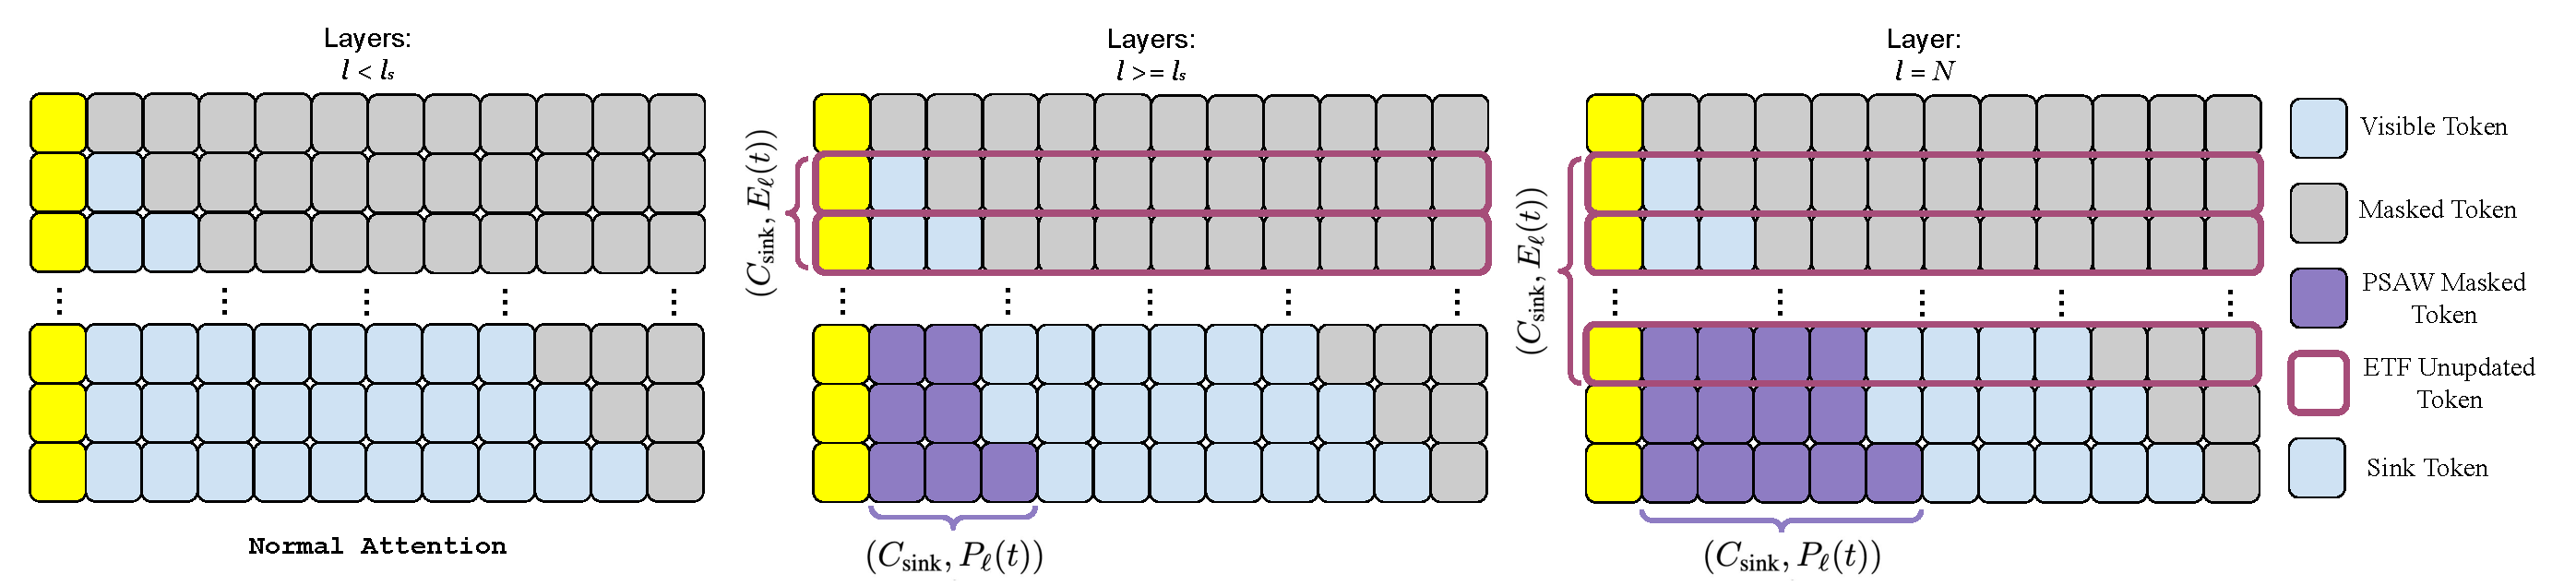
\includegraphics[width=0.95\linewidth]{assets/PSAW-ETF.pdf}
\centering
%\vspace{-0.5em}
    \caption{\textbf{Visual illustration of PSAW and ETF in prefill stage.} When $\ell<\ell_s$, attention is unchanged. For $\ell\ge\ell_s$, both methods prune redundant computation: \textbf{PSAW} computes a per-step sliding window, so the set of \textcolor{PSAW}{masked tokens} can vary across steps (columns); \textbf{ETF} applies a fixed prune range and freezes \textcolor{ETF}{earlier tokens} so they no longer update.}
    \label{fig:psaw&etf}
    \vspace{-0.5em}
\end{figure*}
%------------------------------------------------------


\subsection{Progressive Sliding Attention Window}
\label{sec:psaw}
% \subsubsection{Progressive Sliding Attention Window}

PSAW progressively narrows each layer’s attention window \textbf{during both prefill and decoding}. Consistent with \textbf{Observation~2}, attention is largely localized~\cite{zhang2023h2o,wan2024d2o}: apart from sink tokens, very early tokens receive negligible mass from later queries, and their content has already been propagated forward in lower layers. Thus, attending to them again in deeper layers is redundant.



Let $P_{\ell}(t)$ denote the earliest visible (non-sink) position at step $t$ for layer $\ell$, and let $N$ be the total number of layer. We mask tokens in the index range $(C_{\text{sink}},P_{\ell}(t))$, making the visible set $\{1,\ldots, C_{\text{sink}}\}\cup \{P_{\ell}(t),\ldots,t\}$. Let $\ell_s$ be the layer depth at which pruning starts, we define
\begin{equation}
\label{eq:psaw}
P_\ell(t)=
\begin{cases}
0, &\ell < \ell_s
\\
\big\lfloor (1 \!-\!\phi\;^{\alpha\cdot\frac{\ell-\ell_s}{N-\ell_s}}) \, t \big\rfloor, &\ell \ge \ell_s
\end{cases}
%\;\; \text{where} \;\; \alpha \ge 1 
\end{equation}
where $\phi\!\in\!(0,1)$ and $\alpha\!\ge\!0$. For $\ell\!<\!\ell_s$, no pruning is applied to preserve early-information propagation. For $\ell \!\ge\! \ell_s$, the boundary $P_\ell(t)$ moves monotonically forward with depth because $\phi^{\,\alpha\cdot\frac{\ell-\ell_s}{N-\ell_s}}$ decreases as $\ell$ increases, yielding a progressively shrinking window. We adopt an exponentially decaying schedule rather than a linear one to better match attention locality biases, e.g., positional long-term decay~\cite{su2024roformer} and softmax concentration, yielding tighter alignment with the empirical attention drop in long-range influence across layers (see \textbf{Appendix B}). The parameter $\alpha$ controls the decay schedule, while $\phi^\alpha$ sets the top-layer truncation strength. A visualization of the PSAW mask is shown in Fig.~\ref{fig:psaw&etf}, where \textcolor{PSAW}{tokens in soft violet} indicate masked tokens. 

Theoretically, by assuming attention probability mass with an exponential recency schedule beyond sink tokens, PSAW achieves a design-time certificate $\beta_{\mathrm{th}}^{\mathrm{PSAW}}$ and a tightened MI bound that improves as $\phi^\alpha$ decreases or $\lambda_\ell$ grows.



\subsection{Early Token Freezing}
\label{sec:etf}
During \textbf{prefill}, ETF reduces computation by freezing an expanding prefix of early tokens in deeper layers. The intuition is that information from early tokens has already been propagated forward in shallower layers; further updating them yields diminishing returns. This implementation is also supported by the cross-layer redundancy (Sec.~\ref{sec:intro})~\cite{liu2405minicache}. Let $E_\ell(t)$ denote the last frozen (non-sink) index at layer $\ell$ and step $t$. Tokens with positions in $(C_{\text{sink}},E_\ell(t))$ are excluded from updates: they reuse their previous-layer hidden states, and their attention computations are skipped. Analogous to PSAW, we define
\begin{equation}
\label{eq:etf}
E_\ell(t)=
\begin{cases}
0, &\ell < \ell_s
\\
\big\lfloor (1 \!-\!\psi\;^{\gamma \cdot\frac{\ell-\ell_s}{N-\ell_s}}) \, t \big\rfloor, &\ell \ge \ell_s
\end{cases}
\end{equation}
where $\psi\!\in\!(0,1)$ controls the final unfrozen fraction, and $\gamma\!>\!0$ modulates the nonlinearity of the schedule. A visualization is provided in Fig.~\ref{fig:psaw&etf}, where \textcolor{ETF}{tokens with reddish-purple edges} are frozen. Aligning PSAW, giving a small, depth-decaying budget $\beta_{\mathrm{th}}^{\mathrm{ETF}}$ and a correspondingly tight MI bound, ETF achieves a design-time guarantee by increasing $\ell_s$ or $\mu$, as detailed in \textbf{Appendix D}.


%------------------------------------------------------
\begin{figure}[!t]

\includegraphics[width=0.45\textwidth]{assets/parallel.pdf}
\centering
%\vspace{-1em}
    \caption{\textbf{Parallel CPE acceleration.} \emph{Top:} sequential baseline. \emph{Bottom:} parallel design that fuses index manipulation with attention and directly computes TSA scoring for shared heads. \textcolor{ETF}{ETF masking} will be omitted in decoding.}
    \label{fig:parallel}
    \vspace{-0.5em}
\end{figure}
%--------


\subsection{Parallel Acceleration}

\paragraph{Sequential execution} During inference, CPE executes TSA components in the order shown in Fig.~\ref{fig:parallel} (Top). After KV projection (Eq.~\eqref{eq:qkv-proj}), %\textit{ETF} freezes updates of early tokens (ETF masking is omitted during decoding). 
\textit{ETF} freezes early tokens from further updates; during decoding, explicit ETF masking is unnecessary because only the newly generated position is updated.
Next, \textit{CIS} computes critical sets for shared heads using cosine gating and neighbor dilation (Eqs.~\eqref{eq:cos_sim} and \eqref{eq:neighboring}). We then perform full scoring and build the \textit{PSAW} mask for redundant-attention pruning. For heads that still require retrieval, the top-$k$ oracle is applied to obtain their critical sets. Finally, masks are applied so that each head attends only to its critical set.


\paragraph{Parallel acceleration} Many steps depend only on known quantities and can be prepared or executed in parallel (Fig.~\ref{fig:parallel} (Bottom)). Specifically, previously computed critical sets are cached, and the PSAW mask is query-independent, allowing pre-computation. For CIS-shared heads, critical sets are already known, so full scoring is skipped and we compute attention only over valid indices (TSA scoring). Operations for shared heads and retrieval heads run concurrently, and the overall latency is determined by the slower branch.





